This section contains the implementation details of \toolname{}.
We first describe the implementation and features of the two main components of \toolname{}, the code editor and the GUI editor.
Then, we explain the schema preprocessing steps that are required to generate the GUI editor.
Finally, we describe how we developed a new meta schema for JSON schema that is more suitable for our tool.

\subsection{Technologies}\label{subsec:technologies}

We use vue.js~\cite{vuejsVuejsProgressive} as the UI framework for our tool, combined with the component library PrimeVue~\cite{primevuePrimeVueComponent}.
A detailed list of all libraries used can be found in the wiki of our GitHub repository\footnote{\url{https://github.com/PaulBredl/meta-configurator/wiki/Libraries-we-use}}.
% Table~\ref{tab:libraries} (appendix) shows an overview of the most important libraries used and their purpose.

%\subsubsection{Settings}

% In the Settings view (figure~\ref{fig:settings} in appendix), the user can adjust various parameters (table~\ref{tab:settings} % in appendix) of \toolname{}.


\subsection{Code Panel}\label{subsec:code-editor}

The code editor is a GUI panel designed for editing the \cfgfiles.
For this project, we use the \textit{Ace Editor}\cite{Ace-Editor} library to embed an interactive code editor into our user interface.
It provides useful features for our approach, such as syntax highlighting and code folding.
To make our code editor more user-friendly, we implemented several features, which are described in the following.

\subsubsection{Schema Validation}
To provide the user feedback on whether their data is valid according to the provided schema, we perform schema validation.
We make use of the \textit{Ajv JSON schema validator}\cite{ajv-validator} library, which supports the newest JSON schema draft 2020--12.
%Ajv firstly generates a fast validation function from the input schema.
If schema violations are found, the corresponding user data lines in the code editor will be marked with a red error hint, which also describes the violation.


%\subsubsection{Syntax Highlighting}
%Ace Editor supports syntax highlighting for both JSON and YAML\@.
%With syntax highlighting, the user can easily distinguish between different parts of the data
%and see if the data is syntactically correct.
%% The data format can be switched in the \textit{Settings} page.
%\subsubsection{Collapsing of Code Segments}
%Ace Editor also allows to collapse/expand segments of the text, based on the hierarchical tree structure of the data,
%which allows the user to focus on particular parts of the data.

\subsubsection{Linkage of text with the data model}
As described in section~\ref{subsubsec:design_text_editor_panel}, to map a cursor position in the text editor to
a path in the data model we need to implement the function \texttt{determinePath(editorContent, cursorPosition)}
and to map a path in the data model to a text row in the editor, we need to implement
the function \texttt{determineRow(editorContent, dataPath)}.
% For every data format to be supported, those two functions need to be implemented.

For \textit{JSON}, the functions have been implemented using a \textit{Concrete Syntax Tree (CST)}.
The text content is parsed as a CST.
Then this tree is traversed recursively.
Every tree node has a range property, describing the start and end index of the text belonging to the node.
To determine the corresponding path for a cursor position, the cursor position is translated to a character index
\texttt{targetCharacter} within the text.
Then the CST is traversed and for all nodes \texttt{currentNode} of type array or object for
which \texttt{targetCharacter} $\in$ \texttt{currentNode.range},
the child nodes are checked, and the key of the node (or index for array elements) is appended to the result path.
This way, the corresponding path is built up.

To determine the cursor position for a given path, we reverse this algorithm:
the CST is traversed until the node is found whose path matches the target path.
Then \texttt{currentNode.range.start} is returned as the result index, which is then translated into a cursor position (row and column).

For \textit{YAML}, this linkage is not yet implemented and will be part of further work.

\subsubsection{Editor Operations}
The code editor has more functionalities, such as the possibility to open a file by drag and drop into the editor,
undo/redo operations, and the possibility to change the font size.

\subsection{GUI Panel}\label{subsec:gui-editor}

The GUI editor is a component that allows the user to edit the configuration data in a GUI,
which is generated based on the schema of the configuration data.
It is structured in a table-like way, where each row represents a key-value pair of the configuration data.
Array elements are represented similarly, where the index of the array element is the key and the value is the array element itself.
Figure~\ref{fig:fileeditor} shows the GUI editor component with an example schema and configuration data.

%\begin{figure}[!t]
  %  \centering
 %   \includegraphics[width=\columnwidth]{figures/gui-editor} % todo replace with screenshot => use file editor screenshot?
  %  \caption{GUI Editor Component}
  %  \label{fig:gui-editor}
%\end{figure}

To allow this representation of the schema, we do some preprocessing of the schema,
which is described in section~\ref{subsec:schema-preprocessing}.
To assist the user in editing the configuration data, the GUI editor offers a set of features, which are described in the following.

\subsubsection{Traversal of the Data Tree}
By default, only the first level of the data tree is shown.
The user can expand the data tree by clicking on the arrow next to the key of an object or array.
This will show the sub-properties of the object or the elements of the array.
We limit the depth of the data tree to a configurable value, to prevent the GUI editor becoming too overwhelming.
However, the user can also click on the property name or array index to \textit{zoom in} on that element.
This will show the sub-properties of that element at the top level, as if that property was the root of the data tree.
The breadcrumb at the top allows the user to see which path the GUI editor currently shows and to navigate back to upper levels of the tree.


\subsubsection{GUI implementations for JSON schema features} % Minye
Table~\ref{table:json_schema_type_component} shows how the different JSON schema features are implemented in our GUI\@.
In our GitHub wiki\footnote{\url{https://github.com/PaulBredl/meta-configurator/wiki/JSON-schema-keyword-support}}, we provide a detailed overview of which JSON schema features are supported by our tool.

\begin{table*}[htb]
    \centering
    \caption{Corresponding GUI implementations for JSON schema features\label{table:json_schema_type_component}}
    \begin{tabular}{@{}p{0.2\linewidth}p{0.6\linewidth}@{}}
        \toprule
        \textbf{JSON schema type / keywords} & \textbf{\ GUI implementation} \\
        \midrule
        string & Text field. \\
        number & Text field which allows only floating point numbers and has buttons to increment and decrement. \\
        integer & Text field which allows only integer numbers and has buttons to increment and decrement. \\
        boolean & Checkbox.\\
        object & Expandable list of child columns in the properties table (see figure~\ref{fig:gui_element_object}). \\
        array & Similar as for object.
        Also has a button to add new items (see figure~\ref{fig:gui_element_array}).\\
        enum & Dropdown menu.\\
        const & Dropdown menu with just one entry.\\
        required & Red asterisk left of the property name.\\
        deprecated & Strikethrough styling for property name.\\
        anyOf & Multiselect menu to choose sub-schemas.
        Based on the selected sub-schemas, corresponding properties will be shown as children in the table.\\
        oneOf & Dropdown menu to choose one sub-schema.
        Based on the selected sub-schema, corresponding properties will be shown as children in the table.\\
        \bottomrule
    \end{tabular}
\end{table*}

\begin{figure}[hbt]
    \centering
    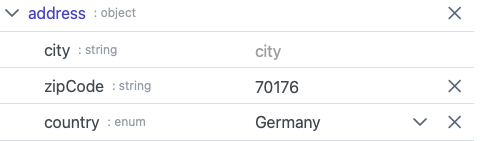
\includegraphics[width=\columnwidth]{figures/gui_element_object}
    \caption{GUI implementation for object properties}
    \label{fig:gui_element_object}
\end{figure}


\begin{figure}[hbt]
    \centering
    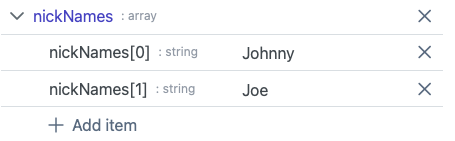
\includegraphics[width=\columnwidth]{figures/gui_element_array}
    \caption{GUI implementation for array properties}
    \label{fig:gui_element_array}
\end{figure}


\subsubsection{Remove Data}
The user can delete properties or array elements from the data by clicking on the $\times$ button next to the edit field.
This button is only shown if the property is not required and there exists data.

\subsubsection{Schema Information Tooltip}
When the user hovers over the property key or array index, an overlay is displayed (figure~\ref{fig:tooltip_example}), which contains all information from the schema about that property.
We manually implemented a generation of a textual description for each of the JSON schema keywords.
Starting with the title and description of the property, the overlay then shows constraints (such as the number must be greater than 0) and at the bottom, it also shows schema violations, in case there are any.
This feature helps the user to understand the constraints and the meaning of a property.

\begin{figure}[hbt]
    \centering
    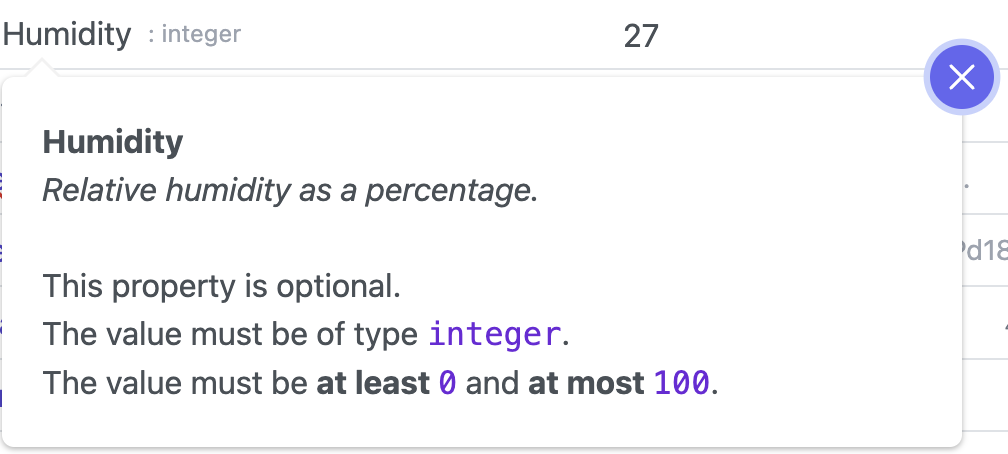
\includegraphics[width=2.5in]{figures/Tooltip_example}
    \caption{Tooltip}
    \label{fig:tooltip_example}
\end{figure}

\subsubsection{Highlighting Schema Validation Errors}
When the configuration data does not comply with the schema, the corresponding elements are underlined in red and highlighted with a red error icon.
This way, the user knows what parts of the data are invalid and what the error is.
Additionally, the schema information tooltip lists all schema violations, as shown in figure~\ref{fig:schema_violation}.

\begin{figure}[hbt]
    \centering
    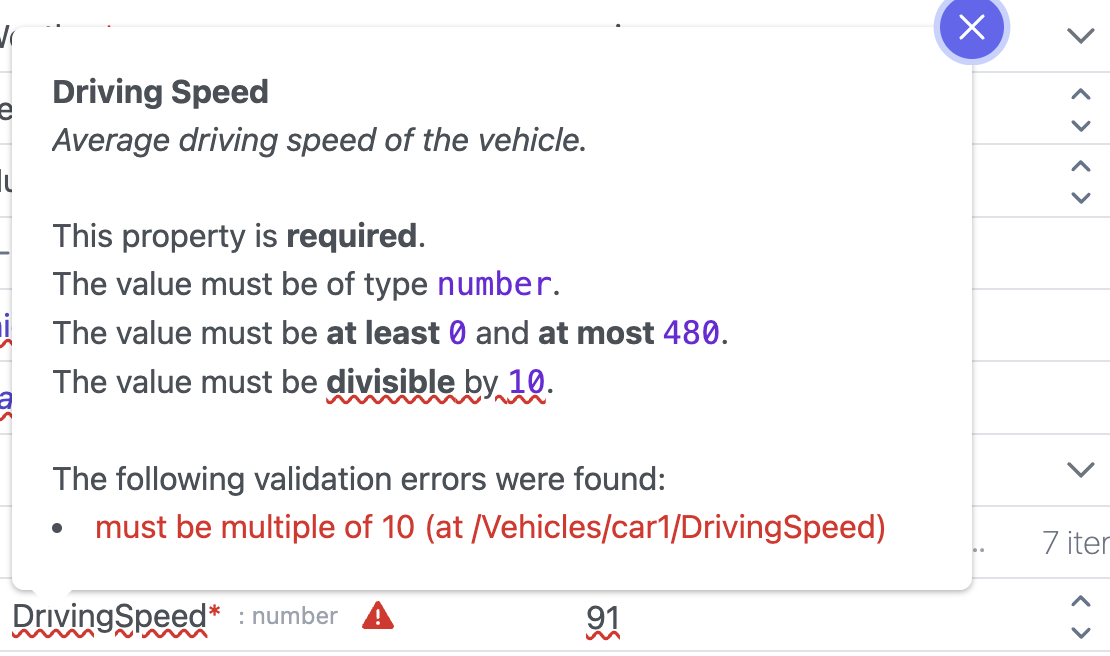
\includegraphics[width=2.5in]{figures/schema_violation}
    \caption{Tooltip with a schema violation}
    \label{fig:schema_violation}
\end{figure}

\subsection{Schema preprocessing}\label{subsec:schema-preprocessing}

To represent the schema in the GUI editor, it is necessary to preprocess the schema as for some JSON schema keywords
it is not immediately clear how to represent them in a GUI\@.
For example, the \texttt{type} keyword can have multiple values, which represents a type union.
There is no obvious GUI component that represents this case.
We differentiate between three ways of preprocessing:
A one-time preprocessing step when loading the schema, an internal preprocessing that happens at every layer of the schema tree,
and calculating an effective schema that happens every time the configuration data changes.
It is important to note that all these preprocessing steps are only used for generating the GUI editor.
They will not affect the schema file itself that is loaded into the schema editor.
The following sections describe the preprocessing steps in detail and how we solve cases like the one just mentioned.

\subsubsection{One-time Preprocessing Step}
When the schema is loaded, we perform a one-time preprocessing step.
This step only processes the whole schema once and does not depend on the configuration data.
We do not perform any time-consuming operations in this step, so the user does not have to wait for the GUI to load.
The following three steps are performed in this preprocessing step:
\begin{enumerate}
    \item Title inducing: If a property does not have the keyword \texttt{title}, we inject the property name as \texttt{title}.
    The \texttt{title} can be then used in various places in the GUI, such as the tooltip as a placeholder in the text field.
    \item Processing \texttt{enum} and \texttt{const}: The \texttt{const} keyword is used to restrict the value of a property to a single value.
    It is semantically equivalent to the \texttt{enum} keyword with a single value.
    Thus, we convert any usage of \texttt{const} to \texttt{enum} with a single element, which allows us to ignore the \texttt{const} keyword in other operations.
    \item Inferring types of enums: If the \texttt{enum} keyword is used, but not the \texttt{type} keyword, we infer the type of the property from the elements of the \texttt{enum} array.
    This is useful for the GUI editor, as it allows us to show the correct type information in the tooltip.
\end{enumerate}

\subsubsection{Lazy preprocessing}
The following preprocessing steps happen at every layer of the schema tree lazily, only when the user expands the corresponding property in the GUI editor.
Laziness of the preprocessing is required as schemas can have circular references, which would, otherwise, lead to infinite loops.
In the following, we describe the preprocessing steps in detail.

\paragraph{Resolving references}
JSON schema uses the \jskeyword{\$ref} keyword to reference other schemas.
This can either be references to schemas in the same file (using the \jskeyword{\$defs} keyword), references to other local files,
or references to schemas at a URL in the web.
We currently only support references to schemas in the same file.
These are lazily resolved as the first preprocessing step.
Listing~\ref{lst:preprocessing-example} shows an example schema, Listing~\ref{lst:reference-resolving} shows the equivalent example after
this first preprocessing step.

\begin{lstlisting}[language=json,firstnumber=1,caption=
    {Simple JSON schema before reference resolving},captionpos=b,label={lst:preprocessing-example}]
{
  "title": "NonEmptyString",
  "$ref": "#/$defs/nonEmptyString",
  "$defs": {
    "nonEmptyString": {
      "type": "string",
      "minLength": 1
     }
  }
}
\end{lstlisting}

\begin{lstlisting}[language=json,firstnumber=1,caption=
    {Simple JSON schema after reference resolving},captionpos=b,label={lst:reference-resolving}]
{
  "allOf": [
   {
     "title": "NonEmptyString"
   },
   {
     "type": "string",
     "minLength": 1
   }
  ],
  "$defs": {
    "nonEmptyString": {
      "type": "string",
      "minLength": 1
     }
  }
}
\end{lstlisting}

\begin{lstlisting}[language=json, firstnumber=1, caption=
    {Simple JSON schema after allOf resolving}, captionpos=b,label={lst:resolved-allof}]
{
  "title": "NonEmptyString",
  "type": "string",
  "minLength": 1,
  "$defs": {
    "nonEmptyString": {
      "type": "string",
      "minLength": 1
     }
  }
}
\end{lstlisting}

\paragraph{Resolving allOfs}

The \jskeyword{allOf} keyword in JSON schema specifies that all the schemas in the given array must be valid.
To simplify any other operation on the schema, we aim to merge the schemas in the \jskeyword{allOf} array into one equivalent schema.
As the first step, we do a recursive step by preprocessing all the schemas of the \jskeyword{allOf} array.
Then, we use the \textit{mergeAllOfs}\cite{githubGitHubMokkabonnajsonschemamergeallof} library to merge all the sub-schemas.
Listing~\ref{lst:resolved-allof} shows the previous example schema after this step.
It is important to note that this library only supports a few keywords of JSON schema, most notably the
\jskeyword{properties} and \jskeyword{items} keyword.
Hence, the \toolname{} has only limited support for \jskeyword{allOf} and any other keywords for which we use this library in the preprocessing.

\paragraph{Converting types to oneOf}
In JSON schema, a property can have multiple types, such as shown in listing~\ref{lst:multiple_types}.
A semantically equivalent schema can be generated by the use of \jskeyword{oneOf}, where each sub-schema contains exactly one of the types,
as shown in listing~\ref{lst:multiple_types_converted}.
If a schema defines more than one type, we convert the types to \texttt{oneOf}.
%This way, we reduce complexity by having to solve only the problem of \jskeyword{oneOf}.
As \texttt{oneOf}s are represented as a dropdown menu in the GUI editor, we now have a way to represent multiple types in the GUI\@.
For schemas that already contain \jskeyword{oneOf}, every type is \textit{multiplied} by every existing \jskeyword{oneOf} sub-schema.
For two types and three \texttt{oneOf} sub-schemas, this will result in a new \texttt{oneOf} with six options.
An exception is when a type can not be merged with a \jskeyword{oneOf} sub-schema (e.g., the \texttt{type} is ``boolean'' and the \texttt{oneOf} sub-schema has type ``string'').
In that case, the incompatible pair is dismissed.

\begin{lstlisting}[language=json, firstnumber=1, caption=
    {Simple JSON schema with three possible types}, captionpos=b, label={lst:multiple_types}]
{
  "type": ["object", "boolean", "string"]
}
\end{lstlisting}

\begin{lstlisting}[language=json, firstnumber=1, caption=
    {Simple JSON schema after conversion of types to oneOf}, captionpos=b,label={lst:multiple_types_converted}]
{
  "oneOf": [
    {
      "type": "object"
    },
    {
      "type": "boolean"
    },
    {
      "type": "string"
    }
  ]
}
\end{lstlisting}


\paragraph{Removing incompatible oneOfs and anyOfs}
A schema may have \jskeyword{oneOf} or \jskeyword{anyOf} options that are not compatible with the schema of the property
(e.g., sub-schemas that can never be fulfilled in combination with the property schema).
Listing~\ref{lst:incompatible_one_ofs} provides an example of a schema with an incompatible \texttt{oneOf} option.
% An example where this occurs is in our adjusted JSON schema meta schema, if we assign the root property the jsonSchema sub-schema, which allows objects and booleans, but then additionally restrict the root to be an object.
For every \jskeyword{oneOf} and \jskeyword{anyOf} sub-schema, we check whether it can be merged with the schema of the property.
The options which are not compatible are removed (see listing~\ref{lst:incompatible_one_ofs_removed}).

\begin{lstlisting}[language=json, firstnumber=1, caption=
    {Simple JSON schema with incompatible oneOf option}, captionpos=b, label={lst:incompatible_one_ofs}]
{
  "type": "object",
  "oneOf": [
    {
      "type": "object"
    },
    {
      "type": "boolean"
    }
  ]
}
\end{lstlisting}


\begin{lstlisting}[language=json, firstnumber=1, caption=
    {Simple JSON schema with the incompatible oneOf option removed}, captionpos=b, label={lst:incompatible_one_ofs_removed}]
{
  "type": "object",
  "oneOf": [
    {
      "type": "object"
    }
  ]
}
\end{lstlisting}


\paragraph{Merging singular oneOfs and anyOfs}
Because of the previous pre-processing step, it can happen that for some \jskeyword{oneOf}s or \jskeyword{anyOf}s, there remains
only one compatible sub-schema left (see listing~\ref{lst:incompatible_one_ofs_removed}).
If this is the case, the use \jskeyword{oneOf}/\jskeyword{anyOf} is redundant, as that singular sub-schema must be chosen implicitly.
Therefore, if there exists only one singular choice for \jskeyword{oneOf}/\jskeyword{anyOf}, we merge its sub-schema into the property schema
and remove the use of \jskeyword{oneOf}/anyOf (see listing~\ref{lst:singular_one_of_merged}).

\begin{lstlisting}[language=json, firstnumber=1, caption=
    {Simple JSON schema with singular oneOf merged into property schema}, captionpos=b, label={lst:singular_one_of_merged}]
{
  "type": "object"
}
\end{lstlisting}


\paragraph{Attempting to merge oneOfs into anyOfs}
Schemas can use both \jskeyword{anyOf} and \jskeyword{oneOf} at the same time.
Especially after converting type unions to \jskeyword{oneOf}, it happens that a schema has \jskeyword{oneOf} options (typically for types) and simultaneously anyOf options.
The user will then have to select both a \jskeyword{oneOf} sub-schema, as well as an \jskeyword{anyOf} sub-schema in the GUI\@.
We observed a special scenario in the JSON meta schema, where the \jskeyword{oneOf} selection was always implicitly given by the \jskeyword{anyOf} selection.
For every single \jskeyword{anyOf} sub-schema, only one \jskeyword{oneOf} sub-schema was compatible.
In that scenario, we can merge the \jskeyword{oneOf}s into the \jskeyword{anyOf}s: for every \jskeyword{anyOf} sub-schema, we merge the one compatible \jskeyword{oneOf} sub-schema into it.
This is precisely what this pre-processing step does: if possible, the \jskeyword{oneOf} sub-schemas are merged into the \jskeyword{anyOf} sub-schemas, and the \jskeyword{oneOf} property is removed from the schema.


\paragraph{Preprocessing oneOfs and anyOfs}
For all remaining \jskeyword{oneOf} and \jskeyword{anyOf} sub-schemas, the internal pre-processing steps are executed.


%\paragraph{Title inducing}
%
%The \texttt{title} keyword is used to give a schema a short description.
%This is not necessarily the same as the property name of properties of an object.
%As we use the title in various cases to display for the user, we inject the property name in cases where no explicit title is given.
%
%\begin{lstlisting}[language=json, firstnumber=1, caption=
%    {Simple JSON schema with one property without a title}, captionpos=b]
%{
%  "type": "object",
%  "properties": {
%    "name": {
%      "type": "string"
%    }
%  }
%}
%\end{lstlisting}\label{listing:no-title}
%
%\begin{lstlisting}[language=json, firstnumber=1, caption=
%    {The property names was used for the title field}, captionpos=b]
%{
%  "type": "object",
%  "properties": {
%    "name": {
%      "title": "name",
%      "type": "string"
%    }
%  }
%}
%\end{lstlisting}\label{listing:with-title}
%
%\paragraph{Processing enum and const}
%The enum keyword is used to restrict the values of a field to a fixed set of valid values.
%The const keyword, similarly, restricts the property value to a single allowed value.
%Thus, setting the const value is equivalent to settings the enum value with an array that contains this single value.
%
%We convert any usage of const to enums with a single element, which allows us to ignore the const keyword in other operations.

\subsubsection{Calculating an effective schema}

This third preprocessing step is calculated every time the data changes.
The JSON schema keywords \texttt{if}, \texttt{then}, and \texttt{else} provide a way to include conditions in the JSON schema.
If the schema in the \texttt{if} field is valid, then also the schema in the \texttt{then} field must be valid, otherwise, the
schema in the \texttt{else} field must be valid.
This makes the schema data dependent.
To show the correct properties, we evaluate the data and dependent on validity or not, we either use the \texttt{then} or the \texttt{else} schema.
We similarly handle the \texttt{dependentRequired} and the \texttt{dependentSchemas} keywords.
For schemas without any of those keywords, this step is trivial as the schema is not modified in any way.

\begin{lstlisting}[language=json, firstnumber=1, caption=
    {Data dependent schema. If the field \texttt{mode} is set to ``manual'' in the data, users will expect that the GUI shows the \texttt{manualValue} property}, captionpos=b, label={lst:ifthen}]
{
  "properties": {
    "mode": {
        "enum": ["manual", "automatic"]
    }
  },
  "if": {
    "properties": {
      "mode": {
        "const": "manual"
      }
    },
    "required": ["mode"]
  },
  "then": {
    "properties": {
        "manualValue": {
            "type": "number"
        }
    }
  }
}
\end{lstlisting}
\begin{lstlisting}[language=json, firstnumber=1, caption=
    {Effective schema when the value for \texttt{mode} is ``manual''}, captionpos=b, label={lst:effectiveschema}]
{
  "properties": {
    "mode": {
        "enum": ["manual", "automatic"]
    },
    "manualValue": {
        "type": "number"
    }
  }
}
\end{lstlisting}

Listing~\ref{lst:ifthen} shows an example of a data-dependent schema and listing~\ref{lst:effectiveschema} shows
the effective schema when the value for \texttt{mode} is ``manual''.

\subsection{Developing a Custom Meta Schema}\label{subsec:schema-editor}

The schema editor view has the same structure as the file editor view, as discussed in previous sections.
The only difference is that the schema used for generating the GUI panel is not the schema file provided by the user but the JSON schema meta schema,
i.e., the schema that defines the structure of valid JSON schema files.
However, applying our generic approach on the official JSON schema meta schema~\cite{jsonschemaJSONSchema} does not result in a user-friendly editor for
creating and modifying schema files.
In this section we discuss the reasons for that and how we developed a new meta schema that circumvents the problems of the official meta schema.

\subsubsection{Missing descriptions}
With the \jskeyword{description} keyword, schema authors can give descriptions to any elements of their schema.
This can help the user of a schema in many ways, for example, the author can specify the unit of a numeric field or give other additional information.
The JSON schema meta schema does not provide any descriptions.
Users, especially those without prior knowledge in JSON schema, might not understand the meaning of the fields of JSON schema.
Thus, we insert descriptions from the JSON schema specification~\cite{jsonschemaJSONSchema} into our modified meta-schema.

\subsubsection{External references}
\toolname{} does not support references to external schemas yet, i.e., references inside the schema to a schema at a specific URL\@.
Also, \toolname{} does not support the \jskeyword{\$vocabulary} keyword.
Both features are used in the JSON schema meta schema, as it is distributed over multiple schema files.
To circumvent that problem, we put all schemas in one schema file into the \jskeyword{\$defs} object and replace the external references with local references.

\subsubsection{Use of dynamic anchors and references}
The JSON schema meta schema uses dynamic references and dynamic anchors.
The difference of those keywords in comparison to the \jskeyword{\$ref} keyword is that they provide a way to dynamically extend the JSON meta schema
at runtime.
For example, one could combine the JSON schema meta schema with an extension that defines how fields should be serialized in XML\@.
We do not support dynamic references and anchors yet.
We replaced all of them by ``non-dynamic'' references using the \jskeyword{\$ref} keyword.

\subsubsection{Allowing each field in each context}
The JSON schema meta schema allows each field in each context.
For example, if the \jskeyword{type} keyword is used and set to \jskeyword{string}, then the \jskeyword{properties} keyword is allowed,
even though it does not make sense in that context.
According to the specification, any validator should ignore the fields that do not make sense in the current context.
Consequently, if the user gets shown all fields that are allowed by the meta schema, they get overwhelmed, although many fields do not make sense in a given context.
This is also a feedback we got from our user study.

\begin{lstlisting}[language=json, firstnumber=1, caption=
    {If condition for array properties. The \texttt{hasTypeArray} is valid if the current property is of type array. The \texttt{arrayProperty} schema defines the properties of an array.}, captionpos=b,label={lst:if-then-else}]
{
  "if": {
    "$ref": "#/$defs/hasTypeArray"
  },
  "then": {
    "$ref": "#/$defs/arrayProperty"
  }
}
\end{lstlisting}

Thus, we added \jskeyword{if} conditions to each field to only show them when they make sense in the current context.
Listing~\ref{lst:if-then-else} shows an example of such an \jskeyword{if} condition.
The relevant properties for arrays are only shown when the current property is of type array.

To even more reduce the amount of fields shown to the user, we also introduce a custom keyword for our own meta schema.
The keyword \jskeyword{advanced} is a boolean field that is set to \texttt{false} by default.
It is wrapped in an \jskeyword{metaConfigurator} object, which is ignored by any validator as it is not part of the JSON schema specification.
We use this wrapper to prevent any other schema extensions from colliding with our keyword.
When set to \texttt{true}, the field is not shown by default, but only when the user expands an \textit{advanced} section that we added to the GUI.
We put all fields that are not required for the basic usage of the schema into the advanced section.
For this, we oriented ourselves on the work of Baazizi et al.~\cite{baazizi2021empirical}, which analyzed the usage of JSON schema keywords in 82,000 JSON schemas.

% TODO screenshots


% paul
%\subsection{JSON schema versions}\label{subsec:json-schema-versions}

%JSON schema has had 10 different drafts over the years, the newest being draft 2020--12~\cite{jsonschemaJSONSchema}.
%In real-world we cannot expect all schemas to have the newest version.
%Baazizi et al.~\cite{baazizi2021empirical} investigated over 82.000 open-source schemas in 2021, where they found that most of them are using draft 4, which was released in 2013.
%As the different drafts are not necessarily compatible with each other, tools supporting one draft become outdated when a new draft releases.
%However, Viotto et al.~\cite{Viotti_Lagoni_2023} provide a library for migration schemas from older versions to the newest draft without loss of information.
%Thus, by using this library, our tool only needs to support the newest draft directly.
%If a user uses a schema from an older draft, we first migrate it to the newest draft internally.
